Le bain initial correspond à un bain oxyde avec une masse initiale de 10 T, une température initiale de 2900 K et une composition de 0.77 UO$_2$ - 0.12 Zr - 0.11 ZrO$_2$ (ratio molaire $R_{U/Zr}$ = 1.3 et degré d'oxydation du zirconium $C_{Zr}$ = 30 \%). La puissance résiduelle constante $\dot{\mathcal{Q}} = 200$ MW est portée par l'espèce uranium U. Une condition adiabatique est imposée sur la couche d'acier liquide hors équilibre du bain (FE.), sinon, pour le bain sous la croûte, la température d'interface pour la couche supérieure est la température de fusion de la croûte. Un profil de flux plat est utilisé pour la projection des flux des différentes couches du bain sur les mailles de le croûte (voir section~\ref{couplage}). Les propriétés physiques des couches du bain sont calculées en fonction de la composition et de la température de la couche par le biais de l'interface disponible dans PROCOR aux lois de propriétés physiques par espèces et des lois de mélanges implantées TOLBIAC-ICB. Enfin, les caractéristiques utiles des différentes couches du bain sont détaillées dans le tableau~\ref{tab:caracteristiques_couches_bain}, en particulier les températures de solidification des couches ainsi que les corrélations de flux de chaleur utilisées pour le calcul des puissances latérales $\phi S$ (voir~\cite{Bonnet1999} ou~\cite{Tourniaire2009a} pour plus de détails sur les corrélations).
\begin{table}
	\centering
	\begin{tabular}{ccc} 
	\hline
	Couche & $\temperature{liq}$ (K) & Corrélation latérale\\
	\hline
	Acier liquide (FE.) & 1600 & ChurchillAndChu\\
	Métal léger (LM.) & 1600 & ChurchillAndChu\\
	Oxyde (OX.) & 3000 & BaliDownWard\\
	Métal lourd (HM.) & 1600 & BaliDownWard\\
	\hline
	\end{tabular}	
	\caption{Configuration initiale du bain de corium pour le test.} 
	\label{tab:caracteristiques_couches_bain}
\end{table}

Enfin, la croûte est divisée, tout au long du calcul, en 20 mailles. La puissance résiduelle constante $\dot{\mathcal{Q}} = 200$ MW dans la croûte est portée par l'espèce uranium U. Le résidu d'apparition de la croûte est de 5 mm. Une température constante et uniforme de 1600 K est imposée sur les parois extérieures de la croûte (seul le couplage entre le modèle de bain de corium et le modèle de croûte sont testés ici).

Différentes coulées d'acier liquide à différents instants du calcul permettent de reproduire des stratifications du bain d'intérêt pour les calculs accidents graves dans le contexte d'IVR. En particulier, ces coulées ont été calculées en fonction du seuil d'inversion de stratification du bain (correspondant à quantité d'acier dans la bain permettant le passage d'un état d'équilibre thermochimique composé d'une couche de métaux lourds en dessous d'une couche d'oxydes vers un équilibre composé d'une couche d'oxydes en dessous d'une couche de métaux légers). Les caractéristiques de ces coulées (temps de début et de fin, masse, température et composition) sont détaillés dans le tableau~\ref{tab:coulees_acier}. 
\begin{table}
	\centering
	\begin{tabular}{ccccc} 
	\hline
	$t_{\text{début}}$ (s) &  $t_{\text{arrêt}}$ (s) & Débit (kg/s) & T (K) & Composition\\
	\hline
	15 000 & 15 200 & 5 & 1605 & 0.687 Fe - 0.208 Cr - 0.106 Ni\\
	30 000 & 30 200 & 8 & 1605 & 0.687 Fe - 0.208 Cr - 0.106 Ni\\
	\hline
	\end{tabular}	
	\caption{Les différentes coulées d'acier liquide imposées pour le test.} 
	\label{tab:coulees_acier}
\end{table}
Un temps suffisamment long entre chacune de ces coulées est imposé pour permettre au bain d'atteindre un état thermique et thermochimique quasi-stationnaire. Les différentes configurations quasi-stationnaires du bain obtenues (OX. puis HM./OX. puis OX./LM.) sont décrites dans la figure~\ref{fig:stratification_bains}.
\begin{figure}
\centering
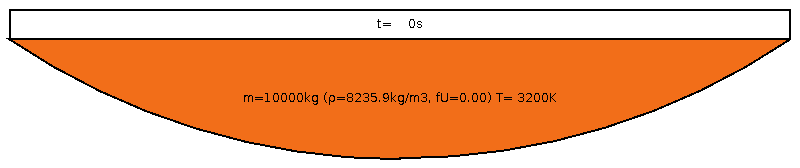
\includegraphics[width=0.8\textwidth, keepaspectratio=true]{Figures/coriumPool_t=00000.png}\\
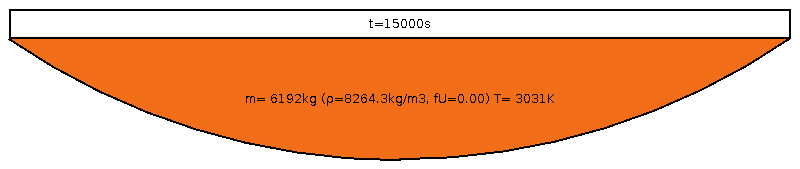
\includegraphics[width=0.8\textwidth, keepaspectratio=true]{Figures/coriumPool_t=15000.png}\\
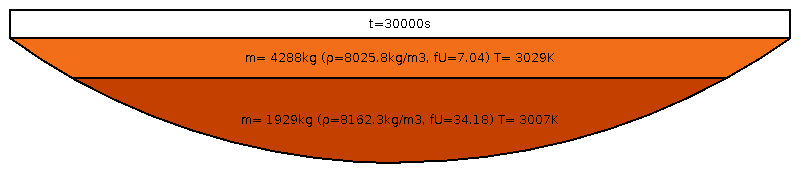
\includegraphics[width=0.8\textwidth, keepaspectratio=true]{Figures/coriumPool_t=30000.png}\\
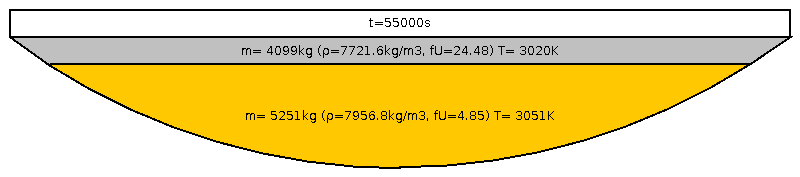
\includegraphics[width=0.8\textwidth, keepaspectratio=true]{Figures/coriumPool_t=55000.png}
\caption{La configuration initiale et les différentes stratifications quasi-stationnaires du bain de corium en fond de cuve atteintes lors du test : \textcolor{orange!75!black}{\textbf{OX.}} à t=15 000 s puis \textcolor{red!50!black}{\textbf{HM.}}/\textcolor{orange!75!black}{\textbf{OX.}} à t=30 000 s puis \textcolor{orange!75!black}{\textbf{OX.}}/\textcolor{orange!50!white}{\textbf{LM.}} à t=55 000 s.}
\label{fig:stratification_bains}
\end{figure}
On notera que, comme le montre la figure, le volume de la croûte est bien pris en compte pour le calcul du volume qu'occupe le bain de corium en fond de cuve de sorte que, hormis lors des coulées d'acier, le mouvement du bain reste relativement faible (et principalement dû aux propriétés physiques dépendantes de la température).

Par la suite, les premiers macro pas de temps du calcul ne seront pas considérés. L'initialisation thermique de la croûte expliquée dans la section~\ref{sect:thermique} permet effectivement d'obtenir un flux externe de croûte initialement nul. Néanmoins, la configuration du couplage thermique entre le bain de corium et la croûte amène le modèle de conduction 0D utilisé à sur-évaluer ce flux externe sur les pas de temps suivants. Néanmoins, au bout de quelques pas de temps (après épaississement de la croûte), le modèle de conduction évalue correctement les différents flux de chaleur de la croûte. Ces difficultés liées au modèle de conduction utilisé dans PROCOR ont déjà été identifiées dans une étude sur la prise en compte de la conduction axiale dans ce modèle dans~\cite{Peybernes2018} et des travaux sont en cours pour les soulever.

Durant les différentes étapes du transitoire, de la masse est échangée entre le bain de corium et sa croûte par solidification du bain ou fusion de la croûte. La figure~\ref{fig:mass_balance} donne les masses des différentes couches du bain de corium et la masse globale de croûte.
\begin{figure}
\centering
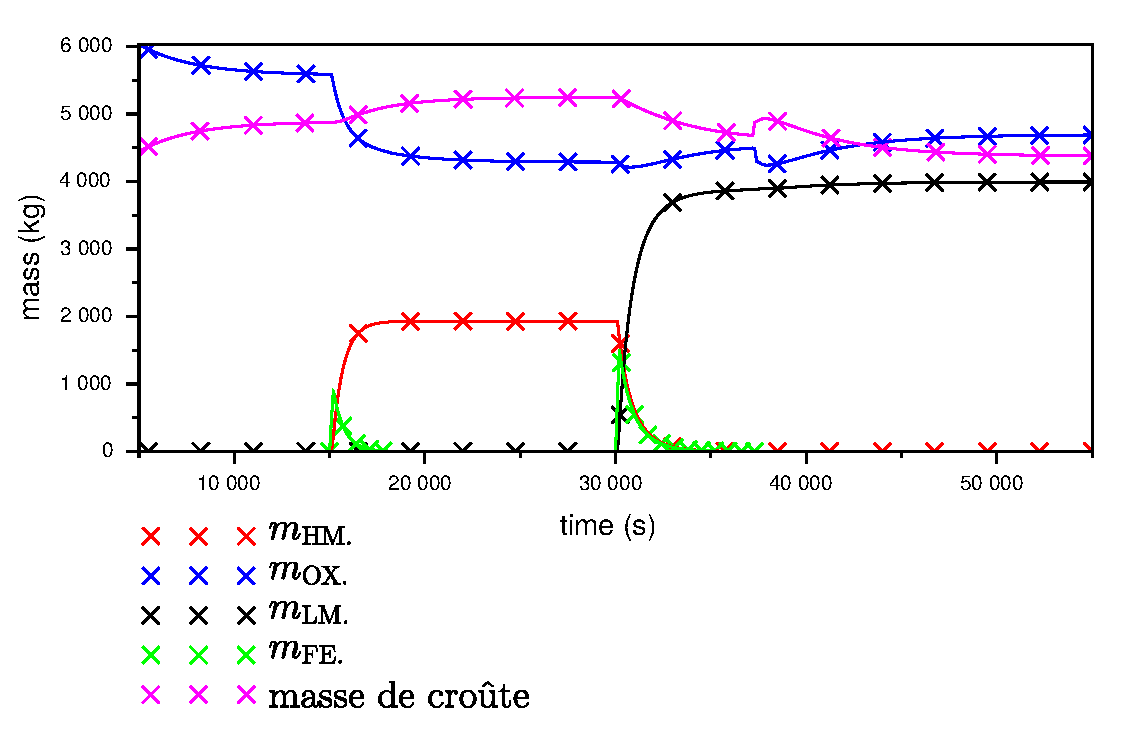
\includegraphics[width=0.85\textwidth, keepaspectratio=true]{Figures/mass_balance.eps}\\
\caption{Masses de la croûte et des couches du bain.}
\label{fig:mass_balance}
\end{figure}
À chaque macro pas de temps du calcul et en fin de calcul, \emph{on vérifie bien la conservation de la masse globale du système}.

De la même manière, de l'énergie est échangée entre le bain de corium et la croûte et \emph{on vérifie la conservation globale de l'énergie du système}. La figure~\ref{fig:thermal_balance} donne les différentes puissances d'intérêt du bain de corium et de la croûte au cours du transitoire.
\begin{figure}
\centering
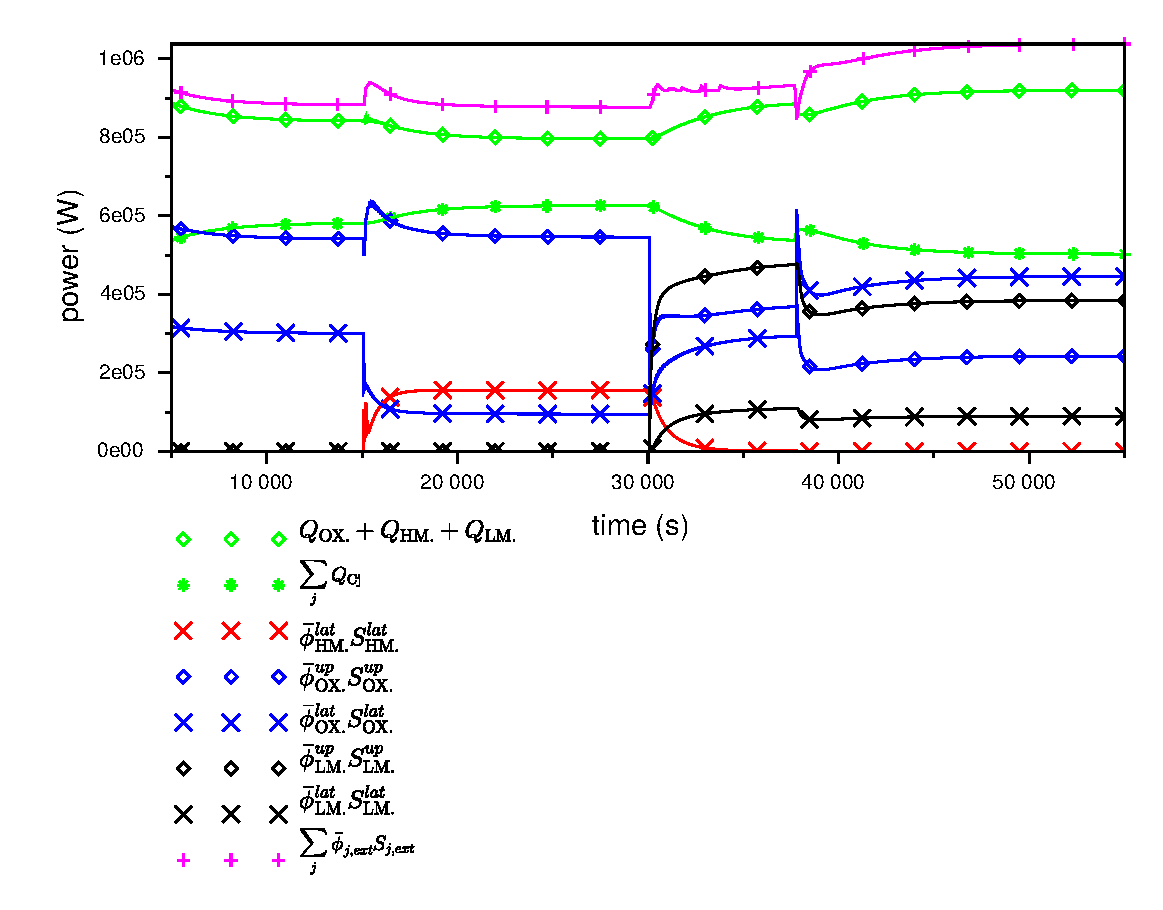
\includegraphics[width=0.85\textwidth, keepaspectratio=true]{Figures/thermal_balance.eps}\\
\caption{Puissances d'intérêt du système bain de corium et croûte.}
\label{fig:thermal_balance}
\end{figure}
En particulier, les puissances évacuées par les surfaces latérales des différentes couches du bain 
\begin{equation*}
\bar{\phi}^{lat}_\textrm{HM.}S^{lat}_\textrm{HM.},\,\bar{\phi}^{lat}_\textrm{OX.}S^{lat}_\textrm{OX.},\,\bar{\phi}^{lat}_\textrm{LM.}S^{lat}_\textrm{LM.}
\end{equation*}
et par sa surface supérieure 
\begin{equation*}
\bar{\phi}^{up}_\textrm{OX.}S^{up}_\textrm{OX.}\quad\text{puis}\quad\bar{\phi}^{up}_\textrm{LM.}S^{up}_\textrm{LM.}\quad\text{pour t $>$ 30 000 s},
\end{equation*}
la somme des puissances résiduelles des couches du bain $Q_\textrm{OX.}+Q_\textrm{HM.}+Q_\textrm{LM.}$ ainsi que la somme des puissances résiduelles $Q_{C_j}$ des mailles $C_j$ de la croûte, et enfin la somme des puissances $\bar{\phi}_{j,ext}S_{j,ext}$ évacuées par la surface extérieure $\gamma_{ext}$ des mailles $C_j$ de la croûte. La conservation de l'énergie peut être vérifiée graphiquement dans la figure~\ref{fig:thermal_balance} aux trois états quasi-stationnaires atteints. Par exemple, pour t=15 000 s, on a :
\begin{equation}
\bar{\phi}^{up}_\textrm{OX.}S^{up}_\textrm{OX.} + \bar{\phi}_{j,ext}S_{j,ext} = Q_\textrm{OX.} + \sum_j Q_{C_j}.
\end{equation}

Durant le transitoire, les mailles de la croûte passent dans les différents états décrits dans la section~\ref{sect:thermique} (solidification, conduction et fusion). En particulier, pour la première partie du transitoire pour t $\leq$ 15 000 s, la croûte se solidifie jusqu'à atteindre un état quasi-stationnaire de solidification (voir figure~\ref{fig:croutes_1}).  
\begin{figure}
\centering
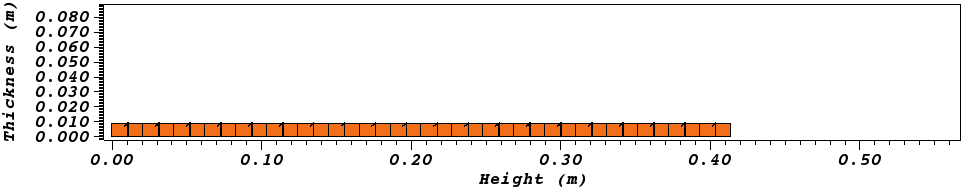
\includegraphics[width=\textwidth, keepaspectratio=true]{Figures/croute_100.png}\\
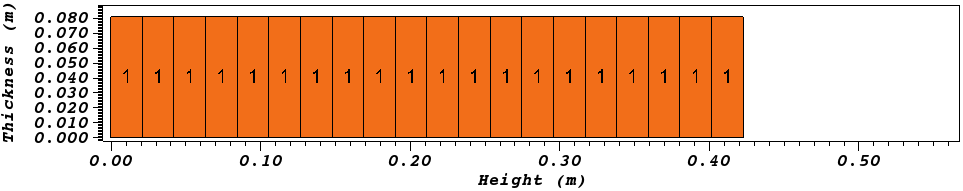
\includegraphics[width=\textwidth, keepaspectratio=true]{Figures/croute_15000.png}
\caption{Croûte à t = 100 s (en haut) et à t = 15 000 s (en bas). \textit{L'indice dans la maille $C_j$ donne la couche de bain en face de celle-ci : 0 $\Leftrightarrow$ HM., 1 $\Leftrightarrow$ OX., 0 $\Leftrightarrow$ LM., 3 $\Leftrightarrow$ FE., -1 $\Leftrightarrow$ pas de contact avec le bain}.}
\label{fig:croutes_1}
\end{figure}

Lors de la seconde partie du transitoire, la couche de métal lourd apparaît suite à une coulée d'acier liquide (voir tableau~\ref{tab:coulees_acier}). La figure~\ref{fig:croutes_2} donne les différents états de la croûte durant ce transitoire.
\begin{figure}
\centering
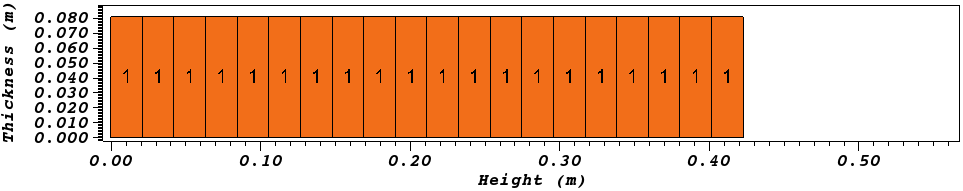
\includegraphics[width=\textwidth, keepaspectratio=true]{Figures/croute_15000.png}\\
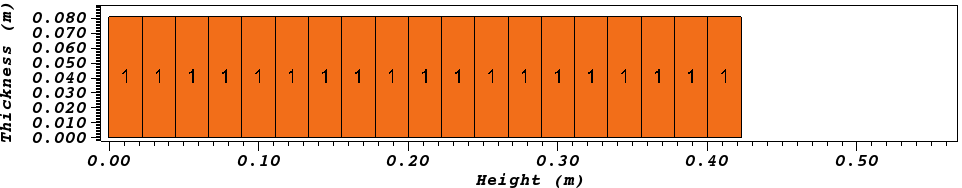
\includegraphics[width=\textwidth, keepaspectratio=true]{Figures/croute_15100.png}\\
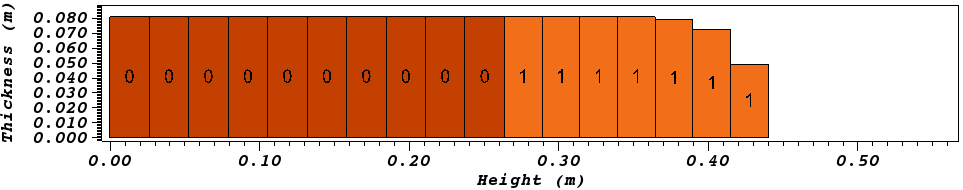
\includegraphics[width=\textwidth, keepaspectratio=true]{Figures/croute_16000.png}\\
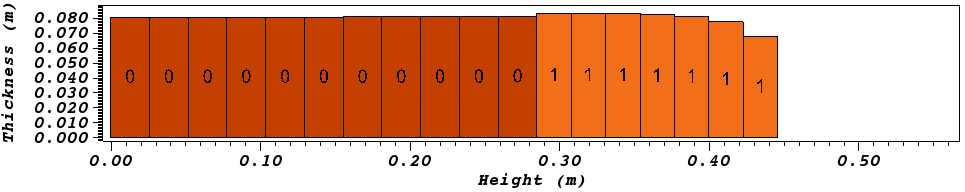
\includegraphics[width=\textwidth, keepaspectratio=true]{Figures/croute_18000.png}\\
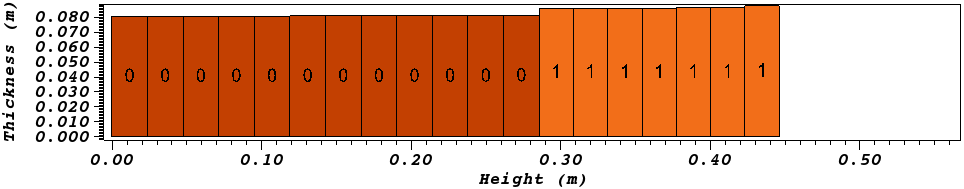
\includegraphics[width=\textwidth, keepaspectratio=true]{Figures/croute_30000.png}\\
\caption{De haut en bas, croûte à t = 15 000 s, t=15 100 s, t=16 000 s, t=18 000 s, t=30 000 s (état quasi-stationnaire du bain HM./OX.). \textit{L'indice dans la maille $C_j$ donne la couche de bain en face de celle-ci : 0 $\Leftrightarrow$ HM., 1 $\Leftrightarrow$ OX., 2 $\Leftrightarrow$ LM., 3 $\Leftrightarrow$ FE., -1 $\Leftrightarrow$ pas de contact avec le bain}.}
\label{fig:croutes_2}
\end{figure}
Entre t=15 000 s et t=15 100 s, une maille de croûte apparaît en face d'une couche d'acier liquide (à une hauteur h $>$ 0.42 m) provenant de la coulée et le maillage de la croûte oxyde passe de 20 mailles (à t=15 000s) à 19 mailles (à t=15 100s). Cette maille de croûte acier apparaît avec une épaisseur initiale de 5 mm mais fond presque instantanément et disparaît. Ensuite, la couche de métal lourd s'épaissit et le volume du bain augmente du fait des propriétés physiques différentes des couches HM. et OX.. Par conséquent, une croûte oxyde apparaît au fur et à mesure (voir les figures à t=16 000 s et t=18 000 s). À t=30 000 s, la thermochimie et la thermique du bain se sont stabilisées et la croûte n'évolue plus : on retrouve bien les profils plats de flux de bain projetés sur les mailles de la croûte.

Enfin, la figure~\ref{fig:croutes_3} donne l'évolution de la croûte pour la dernière partie du transitoire entre t=30 000 s et t=55 000 s.
\begin{figure}
\centering
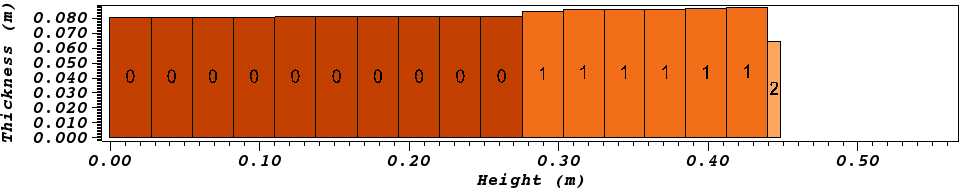
\includegraphics[width=\textwidth, keepaspectratio=true]{Figures/croute_30200.png}\\
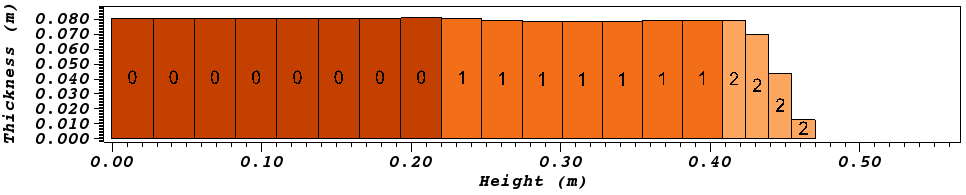
\includegraphics[width=\textwidth, keepaspectratio=true]{Figures/croute_31000.png}\\
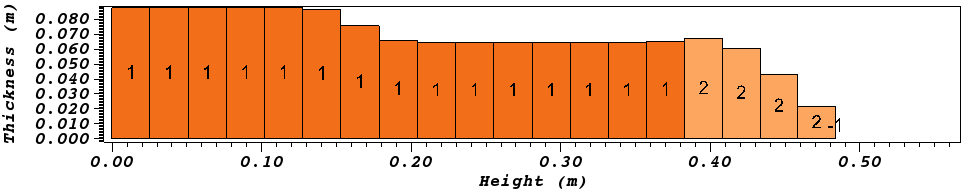
\includegraphics[width=\textwidth, keepaspectratio=true]{Figures/croute_38000.png}\\
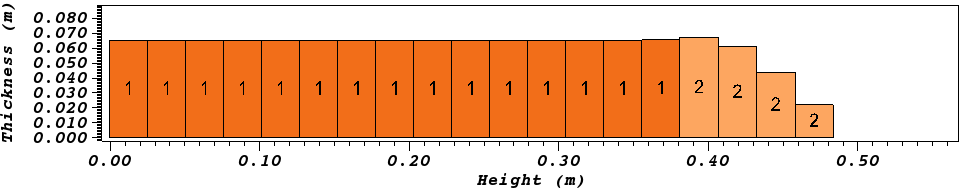
\includegraphics[width=\textwidth, keepaspectratio=true]{Figures/croute_55000.png}
\caption{De haut en bas, croûte à t = 30 200 s, t=31 000 s, t=38 000 s, t=55 000 s (état quasi-stationnaire du bain OX./LM.). \textit{L'indice dans la maille $C_j$ donne la couche de bain en face de celle-ci : 0 $\Leftrightarrow$ HM., 1 $\Leftrightarrow$ OX., 2 $\Leftrightarrow$ LM., 3 $\Leftrightarrow$ FE., -1 $\Leftrightarrow$ pas de contact avec le bain}.}
\label{fig:croutes_3}
\end{figure}
On peut voir l'apparition d'une première maille de croûte en face de la couche métal léger LM. du bain (indice 2 dans la figure). Le volume du bain augmente suite aux coulées d'acier et plusieurs mailles de croûte en face de la couche LM. apparaissent. À t=38 000 s, suite à l'inversion de stratification du bain, la couche de métal lourd HM. disparaît au profit d'une couche oxyde OX.. Par conséquent, les mailles de croûte plus froide précédemment en face de celle-ci passent de l'état conduction à l'état solidification ($\temperature[HM.]{liq} < \temperature[OX.]{liq}$). À t=38 000 s, les premières mailles de croûte sont suffisamment chauffées et repassent en fusion jusqu'à atteindre un état stationnaire à t=55 000 s avec un profil de flux plat du bain.

La figure~\ref{fig:phi_in} donne les flux de chaleur entrant dans les 15 premières mailles de croûte au cours du temps. 
\begin{figure}
\centering
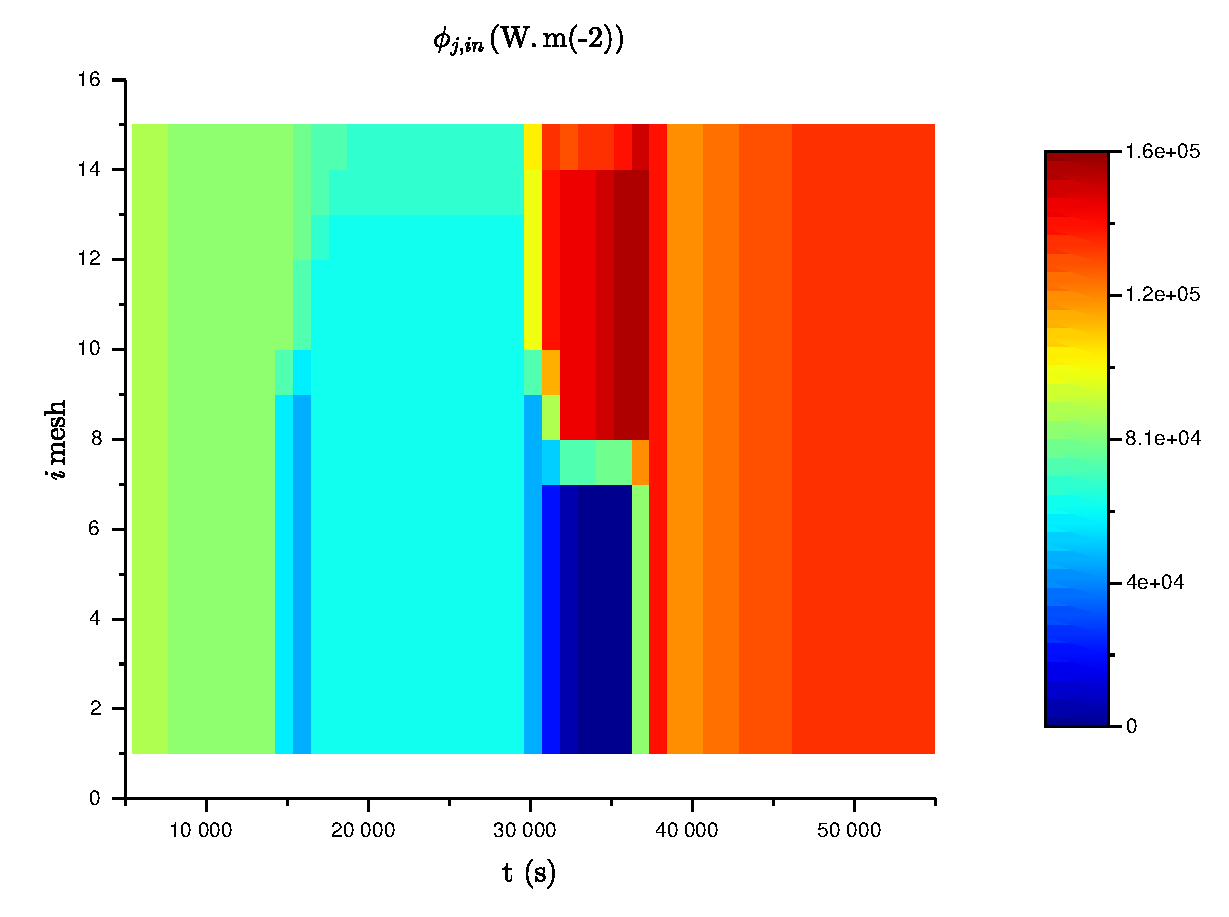
\includegraphics[width=\textwidth, keepaspectratio=true]{Figures/phi_in.eps}
\caption{Flux de chaleur entrant dans la croûte au cours du temps pour les 15 premières mailles de croûte.}
\label{fig:phi_in}
\end{figure}

La figure~\ref{fig:phi_ext} donne les flux de chaleur sortant des 15 premières mailles de croûte du temps.
\begin{figure}
\centering
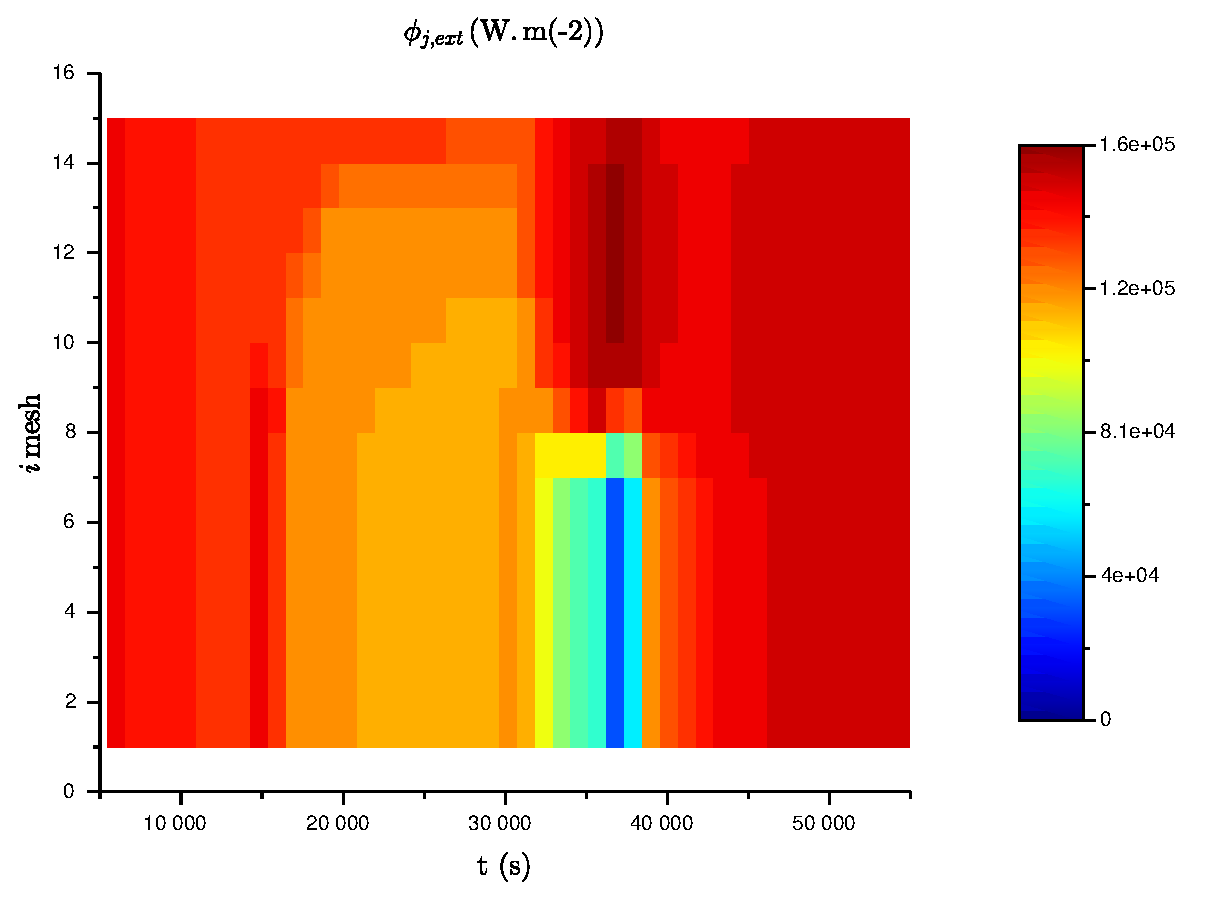
\includegraphics[width=\textwidth, keepaspectratio=true]{Figures/phi_ext.eps}
\caption{Flux de chaleur sortant de la croûte au cours du temps pour les 15 premières mailles de croûte.}
\label{fig:phi_ext}
\end{figure}
